%\documentclass{sig-alternate-draft}
%\documentclass{sig-alternate}\newcommand{\note}[2]{}

% Uncomment to turn on automatic table generation
%\documentclass[preprint]{sig-alternate} % TB 2013-09-15: Modified sig-alternate to include page numbers
%\documentclass[pageno]{jpaper}
%\documentclass[10pt,preprint]{sigalternate}
%\documentclass[10pt,preprint]{sigalternate}
\documentclass[sigconf]{acmart}
\setcopyright{rightsretained}
%\newcommand{\asplossubmissionnumber}{396}

\usepackage[normalem]{ulem}
%\usepackage{siunitx}
\newif\ifsigalt\sigalttrue % false means submission mode.
%\usepackage{supertech-sig}

%begin supertech grap
\pagenumbering{gobble}
\usepackage{clrscode4e}
\usepackage{xspace} % xspace takes care of the \@ after a capitalized word before a period.
\usepackage{amsmath}
\usepackage{subcaption}
\usepackage{afterpage}
\usepackage{placeins}
%\usepackage[x11names]{xcolor}
\usepackage{hyperref}
\hypersetup{
    colorlinks,
    linkcolor={red!50!black},
    citecolor={blue!50!black},
    urlcolor={blue!80!black}
}

% Margin notes - use \notesfalse to turn off notes.
%\newif\ifnotes
%\notestrue
%\newcommand{\longnote}[1]{%
%  \ifnotes
%    {\medskip\noindent Note: \marginpar[\hfill$\Longrightarrow$]
%      {$\Longleftarrow$}{#1}\medskip}
%  \fi}
%
%\newcommand{\cnote}[2]{%
%  \ifnotes%
%  {\scriptsize[[{\color{#1} \sf \raggedright{#2}}]]}%
%  %{\marginpar{\color{#1}\tiny \sf \raggedright\parbox[t]{\columnwidth}{#2}}}%
%  \fi}

%\newcommand{\secput}[2]{\section{\protect\raggedright #2}\label{sec:#1}}
\newcommand{\secput}[2]{\section{#2}\label{sec:#1}}
\newcommand{\defn}[1]       {{\textit{\textbf{#1}}}}
\newcommand{\ang}[1]            {\ifmmode{\mathopen{}\left\langle #1 \right\rangle\mathclose{}}
                                 \else{$\mathopen{}\left\langle${#1}$\right\rangle\mathclose{}$}\fi}


\newcommand{\punt}[1]{}
%% References

\newcommand{\chapref}[1]        {Chapter~\ref{chap:#1}}
\newcommand{\secref}[1]         {Section~\ref{sec:#1}}
%\newcommand{\secref}[1]         {\ref{sec:#1}}
\newcommand{\secreftwo}[2]      {Sections \ref{sec:#1} and~\ref{sec:#2}}
\newcommand{\secrefthree}[3]    {Sections \ref{sec:#1}, \ref{sec:#2}, and \ref{sec:#3}}
\newcommand{\secreffour}[4]     {Sections \ref{sec:#1}, \ref{sec:#2}, \ref{sec:#3}, and~\ref{sec:#4}}
\newcommand{\appref}[1]         {Appendix~\ref{app:#1}}
\newcommand{\figlabel}[1]   {\label{fig:#1}}
\newcommand{\figref}[1]         {Figure~\ref{fig:#1}}
\newcommand{\figreftwo}[2]      {Figures \ref{fig:#1} and~\ref{fig:#2}}
\newcommand{\figrefthree}[3]      {Figures \ref{fig:#1}, \ref{fig:#2}, and~\ref{fig:#3}}

\newcommand{\tabref}[1]         {Table~\ref{tab:#1}}
\newcommand{\stref}[1]          {Step~\ref{st:#1}}
\newcommand{\thmlabel}[1]   {\label{thm:#1}}
\newcommand{\thmref}[1]         {Theorem~\ref{thm:#1}}
\newcommand{\thmreftwo}[2]         {Theorems \ref{thm:#1} and \ref{thm:#2}}
\newcommand{\lemlabel}[1]   {\label{lem:#1}}
\newcommand{\lemref}[1]         {Lemma~\ref{lem:#1}}
\newcommand{\lemreftwo}[2]      {Lemmas \ref{lem:#1} and~\ref{lem:#2}}
\newcommand{\lemrefthree}[3]    {Lemmas \ref{lem:#1}, \ref{lem:#2} and~\ref{lem:#3}}
\newcommand{\lemreffour}[4]     {Lemmas \ref{lem:#1}, \ref{lem:#2}, \ref{lem:#3} and~\ref{lem:#4}}
\newcommand{\corlabel}[1]   {\label{cor:#1}}
\newcommand{\corref}[1]         {Corollary~\ref{cor:#1}}
\newcommand{\correftwo}[2]         {Corollaries~\ref{cor:#1} and~\ref{cor:#2}}
\newcommand{\equref}[1]          {Equation~(\ref{eq:#1})}
\newcommand{\STechEqref}[1] {Equation~(\ref{eq:#1})}
\newcommand{\eqreftwo}[2]       {Equations (\ref{eq:#1}) and~(\ref{eq:#2})}
\newcommand{\ineqref}[1]        {Inequality~(\ref{ineq:#1})}
\newcommand{\ineqreftwo}[2]     {Inequalities (\ref{ineq:#1}) and~(\ref{ineq:#2})}
\newcommand{\invlabel}[1]   {\label{inv:#1}}
\newcommand{\invref}[1]         {Invariant~\ref{inv:#1}}
\newcommand{\invreftwo}[2]      {Invariants~\ref{inv:#1} and~\ref{inv:#2}}
\newcommand{\invrefthree}[3]    {Invariants~\ref{inv:#1}, \ref{inv:#2}, and~\ref{inv:#3}}
\newcommand{\condref}[1]        {Condition~\ref{cond:#1}}
\newcommand{\condreftwo}[2]     {Conditions~\ref{cond:#1} and~\ref{cond:#2}}
\newcommand{\ruleref}[1]        {Rule~\ref{rule:#1}}

\newcommand{\defref}[1]         {Definition~\ref{def:#1}}
\newcommand{\defreftwo}[2]      {Definitions \ref{def:#1} and~\ref{def:#2}}
\newcommand{\defrefthree}[3]    {Definitions \ref{def:#1}, \ref{def:#2}, and~\ref{def:#3}}
\newcommand{\propref}[1]        {Property~\ref{prop:#1}}
\newcommand{\propreftwo}[2]     {Properties~\ref{prop:#1} and~\ref{prop:#2}}
\newcommand{\caseref}[1]        {Case~\ref{case:#1}}
\newcommand{\casereftwo}[2]     {Cases \ref{case:#1} and~\ref{case:#2}}
\newcommand{\caserefthree}[3]   {Cases \ref{case:#1}, \ref{case:#2}, and~\ref{case:#3}}
\newcommand{\caserefrange}[2]   {Cases~\ref{case:#1} through~\ref{case:#2}}
\newcommand{\lilabel}[1]        {\label{li:#1}}
\newcommand{\liref}[1]          {line~\ref{li:#1}}
\newcommand{\Liref}[1]          {Line~\ref{li:#1}}
\newcommand{\lirefs}[2]         {lines \ref{li:#1}--\ref{li:#2}}
\newcommand{\Lirefs}[2]         {Lines \ref{li:#1}--\ref{li:#2}}
\newcommand{\lireftwo}[2]       {lines \ref{li:#1} and~\ref{li:#2}}
\newcommand{\Lireftwo}[2]       {Lines \ref{li:#1} and~\ref{li:#2}}
\newcommand{\lirefthree}[3]     {lines \ref{li:#1}, \ref{li:#2}, and~\ref{li:#3}}
\newcommand{\Lirefthree}[3]     {Lines \ref{li:#1}, \ref{li:#2}, and~\ref{li:#3}}
\newcommand{\lirefrange}[1]     {lines \ref{li:#1(}--\ref{li:#1)}}
\newcommand{\Lirefrange}[1]     {Lines \ref{li:#1(}--\ref{li:#1)}}
\newcommand{\exref}[1]          {Exercise~\ref{ex:#1}}
\newcommand{\princref}[1]       {Principle~\ref{prop:#1}}





%\newtheorem{principle}          {Principle}
%\newtheorem{theorem}            {Theorem}
%\newtheorem{lemma}[theorem]     {Lemma}
%\newtheorem{corollary}[theorem] {Corollary}
%\newtheorem{xample}             {Example}
%\newtheorem{definition}         {Definition}
%\newtheorem{property}           {Property}
%\newtheorem{invariant}[theorem] {Invariant}

%\newcommand{\proof}     {\noindent{\em Proof.}\hspace{1em}}
%\def\squarebox#1{\hbox to #1{\hfill\vbox to #1{\vfill}}}
%\newcommand{\qedbox}            {\vbox{\hrule\hbox{\vrule\squarebox{.667em}\vrule}\hrule}}


%end supertech grap


%\notesfalse


% NOTE(TFK): Change \useautotablefalse to \useautotabletrue to turn
%   on automatic table generation.
\newif\ifuseautotable\useautotablefalse

%\documentclass[9pt,twocolumn]{article}  % required by SPAA submission guidelines

%\usepackage{supertech}
\definecolor{light-gray}{gray}{0.95}

%\usepackage{times}
\usepackage{tabu}
\usepackage{python}
\usepackage{booktabs}
\usepackage{tabularx}
\usepackage{graphicx}
\usepackage{epstopdf}
\usepackage{python}
%\usepackage{subcaption}
\usepackage{breqn}

\usepackage[nodisplayskipstretch]{setspace}
\setstretch{0.85}

\setlength{\belowdisplayskip}{-5pt}
\setlength{\belowdisplayshortskip}{-5pt}


%NOTE(TFK): Commands for decreasing amount of space used in equations.
%\setlength{\thinmuskip}{0mu}
%\setlength{\medmuskip}{0mu}
%\setlength{\thickmuskip}{0mu}
\thinmuskip=0mu
\medmuskip=1mu
\thickmuskip=2mu


%\setlength{\abovecaptionskip}{-2pt}
%\setlength{\belowcaptionskip}{-5pt}

%\usepackage{marginpar}
%\usepackage{caption}

%\captionsetup{width=0.9\columnwidth}
%\captionsetup[figure]{labelfont=bf}
%\usepackage{siunitx}{binary-units}

% American letter size:
%\textwidth6.5in \textheight9in \oddsidemargin 0pt \evensidemargin 0pt
%\topmargin -47pt

% Use this to check space usage sans figures.
%\usepackage[printfigures]{figcaps}

\mark{{}{}}     % Initializes TeX's marks

%\newcommand{\yhnote}[1]{\cnote{purple}{YH: #1}}
%\newcommand{\tknote}[1]{\cnote{orange}{TK: #1}}
%\newcommand{\celnote}[1]{\cnote{blue}{CEL: #1}}
%\newcommand{\tbsnote}[1]{\cnote{red}{TB: #1}}
\newcommand{\yhnote}[1]{}
\newcommand{\tknote}[1]{}
\newcommand{\celnote}[1]{}
\newcommand{\tbsnote}[1]{}

%% Misc
 
\def\pgets{\mathrel{\hspace{1pt}\mbox{$+$$=$}\hspace{1pt}}}
\def\otimesgets{\mathrel{\hspace{1pt}\mbox{$\otimes$$=$}\hspace{1pt}}}
\def\veegets{\mathrel{\hspace{1pt}\mbox{$\vee$$=$}\hspace{1pt}}}
\def\wedgegets{\mathrel{\hspace{1pt}\mbox{$\wedge$$=$}\hspace{1pt}}}
\def\plusplus{\mbox{$+$$+$}}
\def\minusminus{\mbox{$-$$-$}}

%\newcommand{\union}             {\cup}
%\newcommand{\bunion}            {\bigcup}
%\newcommand{\intersect}         {\cap}
%\newcommand{\bintersect}        {\bigcap}

%\newcommand{\degree}[1] {\func{deg}(#1)}


\newcommand{\preds}[1] {\attrib{#1}{pred}}
\newcommand{\succs}[1] {\attrib{#1}{succ}}
\newcommand{\adj}[1] {\attrib{#1}{adj}}
\newcommand{\vertices}[1] {\attrib{#1}{vertices}}
\newcommand{\edges}[1] {\attrib{#1}{edges}}
\newcommand{\vcolor}[1] {\attrib{#1}{color}}
\newcommand{\join}[1] {\attrib{#1}{join}}
\newcommand{\counter}[1] {\attrib{#1}{counter}}

\newcommand{\ffpi}{\ensuremath\pi_{\text{FF}}}
\newcommand{\lfpi}{\ensuremath\pi_{\text{LF}}}
\newcommand{\llfpi}{\ensuremath\pi_{\text{LLF}}}

\newcommand{\lnsqd}{\ln^2\!\!\Delta}
\newcommand{\lncbd}{\ln^3\!\!\Delta}
\newcommand{\lnsqbeta}{\ln^2\!\beta}

\newcommand{\logsqd}{\log^2\!\!\Delta}
\newcommand{\logcbd}{\log^3\!\!\Delta}

\newcommand{\attribp}[2]{\ensuremath{#1\negthinspace\rightarrow\negthinspace\id{#2}}}
\newcommand{\attribbp}[3]{\attribp{#1}{\attribp{#2}{#3}}}

% Names
\newcommand{\prism}{\textcolor{red}{\textup{JP}}\xspace}
\newcommand{\JP}{\textup{JP}\xspace}
\newcommand{\LLF}{\textup{LLF}\xspace}
\newcommand{\SLL}{\textup{SLL}\xspace}
\newcommand{\LF}{\textup{LF}\xspace}
\newcommand{\SL}{\textup{SL}\xspace}
\newcommand{\R}{\textup{R}\xspace}
\newcommand{\FF}{\textup{FF}\xspace}
\newcommand{\SD}{\textup{SD}\xspace}
\newcommand{\ID}{\textup{ID}\xspace}

\newcommand{\cilktrace}{\textup{Trace-R}\xspace}
\newcommand{\set}[1]            {\mathopen{}\{ #1 \}\mathclose{}}
%\punt{
%\usepackage[
%	counters = {theorem},
%	title = {Omitted\ Proofs},
%	abstract, appendix
%]{magicappendix}
%}

%\setlength\belowdisplayskip{0pt} 
%\setlength\belowdisplayshortskip{0pt}
%\setlength\abovedisplayskip{0pt} 
%\setlength\abovedisplayshortskip{0pt}
%\expandafter\def\expandafter\normalsize\expandafter{%
%    \normalsize
%    \setlength\abovedisplayskip{5pt}
%    \setlength\belowdisplayskip{5pt}
%    \setlength\abovedisplayshortskip{5pt}
%    \setlength\belowdisplayshortskip{5pt}
%}

% DOI
%\acmDOI{10.475/123_4}
%
%% ISBN
%\acmISBN{123-4567-24-567/08/06}
%
%%Conference
%\acmConference[WOODSTOCK'97]{ACM Woodstock conference}{July 1997}{El
%  Paso, Texas USA} 
%\acmYear{1997}
%\copyrightyear{2016}
%
%\acmPrice{15.00}

\copyrightyear{2017} 
\acmYear{2017} 
\setcopyright{acmcopyright}
\acmConference{SPAA '17}{July 24-26, 2017}{Washington DC, USA}\acmPrice{15.00}\acmDOI{10.1145/3087556.3087566}
\acmISBN{978-1-4503-4593-4/17/07}


%\copyrightyear{2017} 
%\acmYear{2017} 
%\setcopyright{acmcopyright}
%\acmConference{SPAA'17}{}{July 24--26, 2017, Washington, DC, USA}
%\acmPrice{15.00}
%\acmDOI{http://dx.doi.org/10.1145/XXXXXXX.XXXXXXX}
%\acmISBN{978-1-4503-4593-4/17/07} 
%Authors, replace the red X's with your assigned DOI string. See pdf attached to ACM rightsreview confirmation email.

\fancyhead{}
\settopmatter{printacmref=false}




\makeatletter\begin{document}

%TFKNOTE: See if removing these two lines reduces bad breaks.
%\belowdisplayshortskip=0pt
%\belowdisplayskip=0pt



\title{Optimal Reissue Policies for Reducing Tail Latency}


%\numberofauthors{3}

  %\streetaddress{32 Vassar Street}
  %\city{Cambridge}
  %\state{Massachusetts}
  %\postcode{02139}

\author{Tim Kaler}
\affiliation{
  \vspace{2.5ex}
  \institution{MIT CSAIL}
  %\streetaddress{32 Vassar Street}
  %\city{Cambridge}
  %\state{Massachusetts}
  %\postcode{02139}
}
\email{tfk@mit.edu}

\author{Yuxiong He}
\affiliation{
  \institution{Microsoft Research}
  %\streetaddress{32 Vassar Street}
  %\city{Cambridge}
  %\state{Massachusetts}
  %\postcode{02139}
}
\email{yuxhe@microsoft.com}

\author{Sameh Elnikety}
\affiliation{
  \institution{Microsoft Research}
  %\streetaddress{32 Vassar Street}
  %\city{Cambridge}
  %\state{Massachusetts}
  %\postcode{02139}
}
\email{samehe@microsoft.com}


% \author{%
% Tim Kaler \hspace{2em}
% Yuxiong He \hspace{2em}
% Sameh Elnikety \\\hspace{2em}
%     \url{tfk@mit.edu}\\
%     \url{{yuxhe, samehe}@microsoft.com}\\
%     MIT Computer Science and Artificial Intelligence Laboratory\\
%     32 Vassar Street\\
%     Cambridge, MA\ \ 02139
% }
%
%\date{}

% \conferenceinfo{SPAA'13,} {}
% \CopyrightYear{2013}
% \crdata{}
%\clubpenalty=1000
%\widowpenalty=1000

%\punt{
%\footnotenonumber{This work was supported in part by the National
%  Science Foundation under Grants CNS-1017058, CCF-1162148, and
%  CCF-1314547.  Tao B. Schardl is supported in part by an NSF Graduate
%  Research Fellowship.}
%}

%\thispagestyle{empty}
%\vspace*{-4ex}
%\bigskip
%\centerline{{\bf Keywords}: }

%\category{}{}{}[]
%\terms{}
%\keywords{}
%\end{titlepage}
%\newpage

% New command for autoformatting tables.
% To disable, uncomment the line \renewcommand{\autotable}[1] {}
%\newcommand{\autotable}[1] {\immediate\write18{./autogen.sh "#1" > autogen.tmp}\immediate\input{autogen.tmp}}

%\newcommand{\autotableArg}[2] {\immediate\write18{./autogen.sh "#1" "#2" > autogen.tmp}\immediate\input{autogen.tmp}}
%\ifuseautotable
%\else
%\renewcommand{\autotable}[1] {\input{figure_templates/bin/autogen-#1.tex}}
%\renewcommand{\autotableArg}[2] {\input{figure_templates/bin/autogen-#1-#2.tex}}
%\fi

\newcounter{copnum}
\newcommand{\thecop}{COP \arabic{copnum}}

\newcommand{\Let}{\textbf{let} }

\newcommand{\singleR}{\proc{SingleR}\xspace}
\newcommand{\adaptiveSingleR}{\proc{AdaptiveSingleR}\xspace}
\newcommand{\singleD}{\proc{SingleD}\xspace}
\newcommand{\doubleR}{\proc{DoubleR}\xspace}
\newcommand{\multipleR}{\proc{MultipleR}\xspace}

\newcommand{\varQgeqDN}{Q_{X>d_n}\!\!\left[P_n \right]}
\newcommand{\varQN}{Q\!\!\left[P_n \right]}

\newcommand{\varDNPONE}{d_{n\hspace{-.25ex}{+}\hspace{-.25ex}1}}
\newcommand{\varDNPTWO}{d_{n\hspace{-.25ex}{+}\hspace{-.25ex}2}}
\newcommand{\prob}{\textrm{Pr}}


% Alter some LaTeX defaults for better treatment of figures:
    % See p.105 of "TeX Unbound" for suggested values.
    % See pp. 199-200 of Lamport's "LaTeX" book for details.
    %   General parameters, for ALL pages:
    \renewcommand{\topfraction}{0.9}	% max fraction of floats at top
    \renewcommand{\bottomfraction}{0.8}	% max fraction of floats at bottom
    %   Parameters for TEXT pages (not float pages):
    \setcounter{topnumber}{2}
    \setcounter{bottomnumber}{2}
    \setcounter{totalnumber}{4}     % 2 may work better
    \setcounter{dbltopnumber}{2}    % for 2-column pages
    \renewcommand{\dbltopfraction}{0.9}	% fit big float above 2-col. text
    \renewcommand{\textfraction}{0.07}	% allow minimal text w. figs
    %   Parameters for FLOAT pages (not text pages):
    \renewcommand{\floatpagefraction}{0.7}	% require fuller float pages
	% N.B.: floatpagefraction MUST be less than topfraction !!
    \renewcommand{\dblfloatpagefraction}{0.7}	% require fuller float pages

	% remember to use [htp] or [htpb] for placement


% GNUPLOT: LaTeX picture with Postscript
\begingroup
  \makeatletter
  \providecommand\color[2][]{%
    \GenericError{(gnuplot) \space\space\space\@spaces}{%
      Package color not loaded in conjunction with
      terminal option `colourtext'%
    }{See the gnuplot documentation for explanation.%
    }{Either use 'blacktext' in gnuplot or load the package
      color.sty in LaTeX.}%
    \renewcommand\color[2][]{}%
  }%
  \providecommand\includegraphics[2][]{%
    \GenericError{(gnuplot) \space\space\space\@spaces}{%
      Package graphicx or graphics not loaded%
    }{See the gnuplot documentation for explanation.%
    }{The gnuplot epslatex terminal needs graphicx.sty or graphics.sty.}%
    \renewcommand\includegraphics[2][]{}%
  }%
  \providecommand\rotatebox[2]{#2}%
  \@ifundefined{ifGPcolor}{%
    \newif\ifGPcolor
    \GPcolortrue
  }{}%
  \@ifundefined{ifGPblacktext}{%
    \newif\ifGPblacktext
    \GPblacktexttrue
  }{}%
  % define a \g@addto@macro without @ in the name:
  \let\gplgaddtomacro\g@addto@macro
  % define empty templates for all commands taking text:
  \gdef\gplbacktext{}%
  \gdef\gplfronttext{}%
  \makeatother
  \ifGPblacktext
    % no textcolor at all
    \def\colorrgb#1{}%
    \def\colorgray#1{}%
  \else
    % gray or color?
    \ifGPcolor
      \def\colorrgb#1{\color[rgb]{#1}}%
      \def\colorgray#1{\color[gray]{#1}}%
      \expandafter\def\csname LTw\endcsname{\color{white}}%
      \expandafter\def\csname LTb\endcsname{\color{black}}%
      \expandafter\def\csname LTa\endcsname{\color{black}}%
      \expandafter\def\csname LT0\endcsname{\color[rgb]{1,0,0}}%
      \expandafter\def\csname LT1\endcsname{\color[rgb]{0,1,0}}%
      \expandafter\def\csname LT2\endcsname{\color[rgb]{0,0,1}}%
      \expandafter\def\csname LT3\endcsname{\color[rgb]{1,0,1}}%
      \expandafter\def\csname LT4\endcsname{\color[rgb]{0,1,1}}%
      \expandafter\def\csname LT5\endcsname{\color[rgb]{1,1,0}}%
      \expandafter\def\csname LT6\endcsname{\color[rgb]{0,0,0}}%
      \expandafter\def\csname LT7\endcsname{\color[rgb]{1,0.3,0}}%
      \expandafter\def\csname LT8\endcsname{\color[rgb]{0.5,0.5,0.5}}%
    \else
      % gray
      \def\colorrgb#1{\color{black}}%
      \def\colorgray#1{\color[gray]{#1}}%
      \expandafter\def\csname LTw\endcsname{\color{white}}%
      \expandafter\def\csname LTb\endcsname{\color{black}}%
      \expandafter\def\csname LTa\endcsname{\color{black}}%
      \expandafter\def\csname LT0\endcsname{\color{black}}%
      \expandafter\def\csname LT1\endcsname{\color{black}}%
      \expandafter\def\csname LT2\endcsname{\color{black}}%
      \expandafter\def\csname LT3\endcsname{\color{black}}%
      \expandafter\def\csname LT4\endcsname{\color{black}}%
      \expandafter\def\csname LT5\endcsname{\color{black}}%
      \expandafter\def\csname LT6\endcsname{\color{black}}%
      \expandafter\def\csname LT7\endcsname{\color{black}}%
      \expandafter\def\csname LT8\endcsname{\color{black}}%
    \fi
  \fi
    \setlength{\unitlength}{0.0500bp}%
    \ifx\gptboxheight\undefined%
      \newlength{\gptboxheight}%
      \newlength{\gptboxwidth}%
      \newsavebox{\gptboxtext}%
    \fi%
    \setlength{\fboxrule}{0.5pt}%
    \setlength{\fboxsep}{1pt}%
\begin{picture}(9070.00,2266.00)%
    \gplgaddtomacro\gplbacktext{%
      \csname LTb\endcsname%%
      \put(132,220){\makebox(0,0)[r]{\strut{}$0$}}%
      \put(132,497){\makebox(0,0)[r]{\strut{}$0.1$}}%
      \put(132,774){\makebox(0,0)[r]{\strut{}$0.2$}}%
      \put(132,1051){\makebox(0,0)[r]{\strut{}$0.3$}}%
      \put(132,1328){\makebox(0,0)[r]{\strut{}$0.4$}}%
      \put(132,1605){\makebox(0,0)[r]{\strut{}$0.5$}}%
      \put(159,-77){\rotatebox{45}{\makebox(0,0)[l]{\strut{}$0$}}}%
      \put(449,-77){\rotatebox{45}{\makebox(0,0)[l]{\strut{}$50$}}}%
      \put(739,-77){\rotatebox{45}{\makebox(0,0)[l]{\strut{}$100$}}}%
      \put(1029,-77){\rotatebox{45}{\makebox(0,0)[l]{\strut{}$150$}}}%
      \put(1318,-77){\rotatebox{45}{\makebox(0,0)[l]{\strut{}$200$}}}%
      \put(1608,-77){\rotatebox{45}{\makebox(0,0)[l]{\strut{}$250$}}}%
      \put(1898,-77){\rotatebox{45}{\makebox(0,0)[l]{\strut{}$300$}}}%
    }%
    \gplgaddtomacro\gplfronttext{%
      \csname LTb\endcsname%%
      \put(-220,912){\rotatebox{-270}{\makebox(0,0){\strut{}Mean Maximum \ Relative Error}}}%
      \put(1133,1935){\makebox(0,0){\strut{}ct20stif}}%
      \csname LTb\endcsname%%
      \put(1214,1459){\makebox(0,0)[r]{\strut{}\small PHIL}}%
      \csname LTb\endcsname%%
      \put(1214,1294){\makebox(0,0)[r]{\strut{}\small OSKI}}%
    }%
    \gplgaddtomacro\gplbacktext{%
      \csname LTb\endcsname%%
      \put(2399,220){\makebox(0,0)[r]{\strut{}$0$}}%
      \put(2399,497){\makebox(0,0)[r]{\strut{}$0.1$}}%
      \put(2399,774){\makebox(0,0)[r]{\strut{}$0.2$}}%
      \put(2399,1051){\makebox(0,0)[r]{\strut{}$0.3$}}%
      \put(2399,1328){\makebox(0,0)[r]{\strut{}$0.4$}}%
      \put(2399,1605){\makebox(0,0)[r]{\strut{}$0.5$}}%
      \put(2426,-77){\rotatebox{45}{\makebox(0,0)[l]{\strut{}$0$}}}%
      \put(2716,-77){\rotatebox{45}{\makebox(0,0)[l]{\strut{}$50$}}}%
      \put(3006,-77){\rotatebox{45}{\makebox(0,0)[l]{\strut{}$100$}}}%
      \put(3296,-77){\rotatebox{45}{\makebox(0,0)[l]{\strut{}$150$}}}%
      \put(3585,-77){\rotatebox{45}{\makebox(0,0)[l]{\strut{}$200$}}}%
      \put(3875,-77){\rotatebox{45}{\makebox(0,0)[l]{\strut{}$250$}}}%
      \put(4165,-77){\rotatebox{45}{\makebox(0,0)[l]{\strut{}$300$}}}%
    }%
    \gplgaddtomacro\gplfronttext{%
      \csname LTb\endcsname%%
      \put(3400,1935){\makebox(0,0){\strut{}gupta1}}%
    }%
    \gplgaddtomacro\gplbacktext{%
      \csname LTb\endcsname%%
      \put(4667,220){\makebox(0,0)[r]{\strut{}$0$}}%
      \put(4667,407){\makebox(0,0)[r]{\strut{}$0.5$}}%
      \put(4667,594){\makebox(0,0)[r]{\strut{}$1$}}%
      \put(4667,781){\makebox(0,0)[r]{\strut{}$1.5$}}%
      \put(4667,969){\makebox(0,0)[r]{\strut{}$2$}}%
      \put(4667,1156){\makebox(0,0)[r]{\strut{}$2.5$}}%
      \put(4667,1343){\makebox(0,0)[r]{\strut{}$3$}}%
      \put(4667,1530){\makebox(0,0)[r]{\strut{}$3.5$}}%
      \put(4694,-77){\rotatebox{45}{\makebox(0,0)[l]{\strut{}$0$}}}%
      \put(5042,-77){\rotatebox{45}{\makebox(0,0)[l]{\strut{}$200$}}}%
      \put(5389,-77){\rotatebox{45}{\makebox(0,0)[l]{\strut{}$400$}}}%
      \put(5737,-77){\rotatebox{45}{\makebox(0,0)[l]{\strut{}$600$}}}%
      \put(6084,-77){\rotatebox{45}{\makebox(0,0)[l]{\strut{}$800$}}}%
      \put(6432,-77){\rotatebox{45}{\makebox(0,0)[l]{\strut{}$1000$}}}%
    }%
    \gplgaddtomacro\gplfronttext{%
      \csname LTb\endcsname%%
      \put(5668,1935){\makebox(0,0){\strut{}pathological_oski}}%
    }%
    \gplgaddtomacro\gplbacktext{%
      \csname LTb\endcsname%%
      \put(6934,220){\makebox(0,0)[r]{\strut{}$0$}}%
      \put(6934,374){\makebox(0,0)[r]{\strut{}$0.02$}}%
      \put(6934,528){\makebox(0,0)[r]{\strut{}$0.04$}}%
      \put(6934,682){\makebox(0,0)[r]{\strut{}$0.06$}}%
      \put(6934,836){\makebox(0,0)[r]{\strut{}$0.08$}}%
      \put(6934,989){\makebox(0,0)[r]{\strut{}$0.1$}}%
      \put(6934,1143){\makebox(0,0)[r]{\strut{}$0.12$}}%
      \put(6934,1297){\makebox(0,0)[r]{\strut{}$0.14$}}%
      \put(6934,1451){\makebox(0,0)[r]{\strut{}$0.16$}}%
      \put(6934,1605){\makebox(0,0)[r]{\strut{}$0.18$}}%
      \put(6961,-77){\rotatebox{45}{\makebox(0,0)[l]{\strut{}$0$}}}%
      \put(7251,-77){\rotatebox{45}{\makebox(0,0)[l]{\strut{}$500$}}}%
      \put(7541,-77){\rotatebox{45}{\makebox(0,0)[l]{\strut{}$1000$}}}%
      \put(7831,-77){\rotatebox{45}{\makebox(0,0)[l]{\strut{}$1500$}}}%
      \put(8120,-77){\rotatebox{45}{\makebox(0,0)[l]{\strut{}$2000$}}}%
      \put(8410,-77){\rotatebox{45}{\makebox(0,0)[l]{\strut{}$2500$}}}%
      \put(8700,-77){\rotatebox{45}{\makebox(0,0)[l]{\strut{}$3000$}}}%
    }%
    \gplgaddtomacro\gplfronttext{%
      \csname LTb\endcsname%%
      \put(4580,-330){\makebox(0,0){\strut{}Time to Estimate (in SpMV time)}}%
      \put(7935,1935){\makebox(0,0){\strut{}pathological_asx}}%
    }%
    \gplbacktext
    \put(0,0){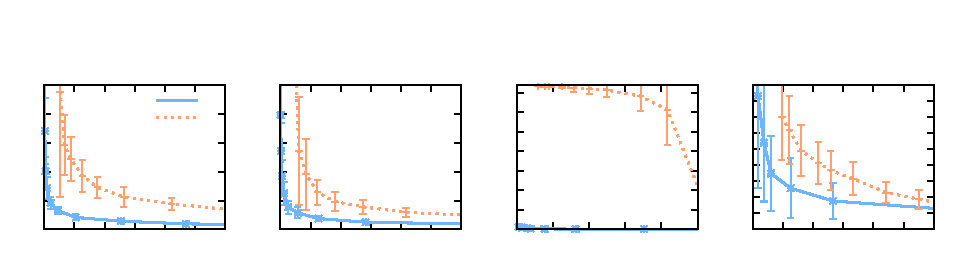
\includegraphics{figures/scanserialvar}}%
    \gplfronttext
  \end{picture}%
\endgroup


%\input{abstract}
%
%\maketitle
%
%%\fontsize{10}{12}\selectfont
%% !TEX root =  main.tex

\section{Introduction}

  We present an algorithm to efficiently compute an important heuristic for autotuning sparse tensor operations. A tensor is a multidimensional array~\cite{KoldBa09}.  A sparse tensor is a tensor whose entries are mostly zeros, which do not have to be stored or operated on in most linear algebraic operations. Since sparse tensors typically contain more than 90\% zero entries, taking advantage of sparsity can provide substantial increases in performance. However, the increased complexity of datastructures that can describe the irregular locations of nonzeros in these tensors poses a significant challenge to performance engineers.

These challenges are magnified in an era of increasing heterogeneity of processors. In order to write the most efficient sparse tensor code, the programmer must take into account both the target architecture and the relevant structural properties of the nonzeros of the sparse tensor. Writing custom code for each processor requires extensive engineering effort and the structure of nonzeros is usually known only at runtime. Therefore, autotuning (automatically generating customized code) has become a necessary part of writing efficient sparse code.

  Previous efforts in autotuning for sparse tensors focus on sparse matrices, which are more broadly applicable in fields ranging from scientific computing to machine learning. The diverse space of operations and nonzero patterns of sparse matrices have led to the development of a wide variety of sparse matrix formats that allow programmers to more efficiently operate on the matrices. 
  
  We limit our description to perhaps the most popular such format, Compressed Spfarse Row (CSR) and a variant we will call Blocked Compressed Sparse Row (BCSR)~\cite{BuluFiFr09}. In CSR, only the nonzeros and their locations are stored in each row of the matrix. In Blocked Compressed Sparse Row, an $m \times n$ matrix is divided into $m/r \times n/c$ submatrices, where each submatrix is of size $r \times c$. The submatrices are called blocks, and are stored in a dense format (so zeros are represented explicitly). Only blocks which contain nonzeros are stored, and the locations of nonzero blocks are stored in CSR format. We only need to store the location of the entire block, instead of individual entries. If many nonzeros appear within the same block, storing the locations of nonzero blocks requires less memory and less computational logic than storing the locations of the individual nonzeros. For matrices that naturally have a block structure of nonzeros, such as those produced by finite element methods, this can improve the performance of sparse matrix operations.

  Given the definition of BCSR, it is natural to wonder how one might choose the correct block size for a given matrix. If we set the block size too small, then we must store the locations of more blocks. If we set the block size too large, then the blocks will be filled with too many zeros.
  Vuduc et. al. describes an effective heuristic for predicting the performance $P$ (in $Mflop/s$) of a particular block size on a sparse matrix $A$.
  We refer to the number of nonzeros in $A$ as $k(A)$. We refer to the number of blocks of size $r \times c$ which contain nonzeros in $A$ as $k_{r, c}(A)$.
  We can then define the \textit{fill} of the matrix to be $f(A) = rck_{r, c}(A)/k(A)$.
  Once per machine, we compute a profile of how the machine performs for a particular block size.
  Let $P_{rc}(dense)$ be the performance of the machine (in $Mflop/s$) on a dense matrix stored with block size $r \times c$.
  Then we can estimate $P_{rc}(A)$ as

  \[
    \tilde{P}_{rc}(A) = \frac{P_{rc}(dense)}{f_{rc}(A)}
  \]

  Thus, our task is to compute $f_{rc}$ for all $r$ and $c$ to within some tolerable relative accuracy, and to do so efficiently. Statistical sampling methods given by Vuduc et. al. provide no theoretical guarantee of accuracy, and take as long as 1 to 10 times the time it takes to perform a sparse matrix vector multiplication on the same matrix~\cite{vuduc04}. We describe an algorithm which provides estimates to within $\epsilon$ relative error with probability $1 - \delta$ in time \todo{$O(\log(\delta)/\epsilon^2)$}, and show that our algorithm runs efficiently and accurately on real-world cases. Note that our algorithm depends only on the desired accuracy, whereas the algorithm introduced by Vuduc et al.\ depends linearly upon the number of nonzeros.

  Our algorithm estimates a more general notion of fill for tensors, where we divide the tensor into smaller subarrays (our blocks) and again only the nonzero blocks and their locations are stored in each row of the tensor. We further generalize this by allowing the user to offset the grid of blocks by some fixed amount, so that the block structure of the tensor does not have to align with the block size.

  Finally, we note that estimating the fill can be an important part of any sparse datastructure which uses blocking, not just BCSR. In fact, any sparse datastructure can be adapted to a blocked regime by grouping a tensor into blocks and simply treating nonzero blocks as nonzeros of some sparse tensor.

%
%%\input{formulation}
%%\input{deterministic}
%\input{random}
%\input{optimality}
%
%%\input{independent}
%%\input{datadriven}
%%\input{datadriven}
%%\input{correlation}
%%\input{aggregation}
%\input{usingsingleR}
%\input{simulation_figure_page}
%\input{simulation_figure_page2}
%\input{eval}
%\input{sensitivity}
%\input{system_figure_page}
%\input{systemeval}
%%% !TEX root =  main.tex

\section{Previous Work}
% \todo{finish plz. Mainly this is Vuduc}Vuduc thesis~\cite{vuduc04}
Fill estimation is an important intermediate step for matrix computation optimization. 
Specifically, it is commonly used in autotuning for sparse matrices to find the
optimal blocking scheme for sparse matrix-vector multiplication~\cite{WillOlVu09, VuducDeYe02, YilmAkGa16, VuducMo05}.
Previous work also includes autotuning for matrix computations on 
GPUs~\cite{ChoiSiVu10} and performance tuning for sparse matrix kernels~\cite{ImYeVu04, ImYe01}. 

To our knowledge, there has not been much theoretical work on the accuracy guarantees of fill estimation methods. We will describe
a sampling-based algorithm in section~\ref{algorithm} for sampling from the nonzero elements of a sparse matrix and
and show its accuracy bounds.

\subsection{Heuristic for fill estimation}

To our knowledge, there are no guarantees on the accuracy existing algorithms for fill estimation. The best known heuristic (due to Vuduc~\cite{vuduc04}) for computing the fill uses randomization, and does not calculate the optimal fill for offsets --- it only estimates the fill for block size pairs $(r,c)$. Furthermore, there is only an empirical study of the cost-accuracy tradeoff in fill estimation. At a high level, the algorithm tests all possible block sizes $(r,c)$ by looping through all possible row dimensions $r$ and dividing the matrix into $m/r$ ``row columns'', each composed of $r$ consecutive row. That is, the $i$-th ``row column'' is rows $ri$ through $r(i+1)-1$.

For a fixed $r$, the algorithm randomly chooses (with probability $\sigma$) to evaluate a ``block row''. That is, it flips a coin (potentially biased) to determine whether or not to process a block row. In order to process a block row, it processes all non-zero elements by setting a relevant bit to keep track of which blocks have already been counted. The algorithm also counts how many nonzeros it has processed and the number of non-empty blocks found in each possible blocking scheme.

The heuristic returns the maximum fill as the sample optimum blocking scheme.

 \begin{samepage}
    \begin{alg}
      Given a sparse matrix of dimensions $m \times n$ and $B$, estimate the fill by evaluating a subset of the rows in each matrix
      \begin{algorithmic}[1]
        \Function{Oski Heuristic}{matrix $A$ (dimensions $m \times n$), max block size $B$, evaluation probability $\sigma$} \\
       \State \texttt{max\_fill} $\gets$ max fill
       \State \texttt{best\_pair} $\gets \emptyset$
          \For{$r = 1 \to B$}
          \State array \texttt{num\_blocks[1:$B$]} $\gets$ 0
          \State \texttt{nnz\_visited} $\gets$ 0
          \For{i from [1, m/r]}
          \State flip a coin with heads probability $\sigma$
          \State array \texttt{last\_block\_index}[1:B] $\gets -1$
          \If the coin came up heads
          \For{nonzero $A(i,j) \in A(ir, (i+1)r-1)$}
          \State \texttt{nnz\_visited} $\gets$ \texttt{nnz\_visited} + 1
          \For{$c = 1 \to B$}
          \State \texttt{last\_block\_index}[c] $\gets j/c$
          \State array \texttt{num\_blocks}[c] $\gets$ \texttt{num\_blocks}[c] + 1
          \EndFor
          \EndFor
          \EndIf
          \EndFor
          \State $\hat{f}_{r,c}(A, \sigma) \gets rc\texttt{num\_blocks}[c]  /  \texttt{nnz\_visited} $
          \EndFor
        \EndFunction
      \end{algorithmic}
      \label{alg:oski}
    \end{alg}
    \end{samepage}

According to the empirical study presented in~\cite{vuduc04}, the algorithm almost always find a blocking
scheme that achieves within 5\% of the optimal (brute force) algorithm. 

\subsection{Asymptotic Runtime Analysis}
Let $k(A)$ be the number of nonzeros in $A$. To estimate the cost to test a single row $r$, we consider the loops.
We expect to estimate the outer loop (choosing a block row) $\sigma m/r$ times. There are $k/m$ nonzeros
per row on average for $rk/m$ nonzeros per block row on average. Therefore, the cost to do fill 
estimation for all possible values of $c$ for one value of $r$ is $$O\left(B\sigma \frac{m}{r} \frac{rk}{m}\right) = O(Bk\sigma). $$

The cost to estimate for all $B$ values of $r$ is therefore $O(B^2k\sigma).$ The expected cost is
linear in $k$ and asymptotically the same as a sparse matrix vector multiply.
%\input{concl}

%\input{appendix}


%\bibliographystyle{abbrv}
\bibliographystyle{ACM-Reference-Format}
\bibliography{allpapers}

\end{document}

%%% Local Variables: 
%%% mode: latex
%%% TeX-master: t
%%% End: 




